To validate our method we will run the alignment approach of task tree generation against the same case study as Harms et al. did.
The data was collected on an application portal of the university.
Figure \ref{fig:screenshotmasterportal} shows a screenshot of the first page of the portal.
After login, users can fill out multiple forms regarding their personal data as well as upload their CVs.
In this case study 555 user created arround 3602 appropriate user sessions.
Further details about the data are enlisted in table \ref{tab:casestudy2}.
The data of the traces is XML structured. Figure \ref{fig:xml} shows the format of one \textit{onclick} event.

\begin{figure}
	
\includegraphics[width=\textwidth]{chapters/casestudy/masterportalscreenshot.png}
	\caption{Screenshot of the website the data was collected with.}
	\label{fig:screenshotmasterportal}
\end{figure}
\begin{figure}
\begin{verbatim}
<event type="onclick">
      <param name="timestamp" value="1389109340615"/>
      <param name="target" value="DSuS8oahm5 ... NfhupVDJCn=="/>
      <param name="Y" value="64"/>
      <param name="X" value="662"/>
</event>
\end{verbatim}
\caption{Example of one event in XML structure}
\label{fig:xml}
\end{figure}



\begin{table}
	\centering
	 \begin{tabular}{|r|c|}
		   \hline
		   & \textbf{Application Portal }\\
		     \hline
		       Start of Recording & 25 October 2013 \\
		       End of Recordning & 7 March 2014 \\
		       Recorded Users & 555 \\
		       Recorded User Sessions & 4,129 \\
		       Considered User Sessions & 3,602 \\
		       \hline
		         \textbf{Recorded Events} & 350,368 \\
		         Relevant Events & 306,568 \\
		         Double Clicks & 6,437 \\
		         Focus Changes & 89,825 \\
		         \hline
			   \textbf{Considered Events} & 210,306 \\
			   Different Events & 1,897 \\
			   \hline
			    \end{tabular}
			    \caption{Case study overview}
	\label{tab:casestudy2}
\end{table}

We are interested in several aspects of the task tree creation with the alignment approach.
First of all we want to examine the necessity of the calculation of the distance between non-event-tasks.
The calculations of those distances are very expensive operations so we want to know if this step could be left out and we still find approximately the same amount of tasks in the same quality.
After that we study the algorithms termination conditions with the goal to find out if we can terminate the algorithm earlier than proposed in chapter \ref{chap:approach}.

Afterwards, we evaluate the performance of the alignment approach and compare it to the performance of the n-gram approach.
At last we discuss the created task tree by means of representative task examples after running the alignment approach on the full case study.
All experiments were executed on a AMD Opteron(TM) Processor 6276 (64 core) with 250GB of ram after we figured out, that a Intel(R) Core(TM) i5-2520M CPU @ 2.50GHz with 8GB of ram is not sufficient to run the alignment approach on large numbers of user sessions.
The Java virtual machine was started with the following parameters:
\begin{itemize}
	\item -XX:+UseConcMarkSweepGC
	\item -Xmx84000m
\end{itemize}

\section{Parameters}
The alignment approach has several parameters that have to be set before running the algorithm. Some values of the parameters may also depend on the underlying data.
All parameters are described in the approach chapter. Table \ref{tab:parameters} gives a short summary of all available parameters that can be set and also the values
we used in this case study. Those parameters were manually chosen by trial and error and do not guarantee the best possible results.

\begin{table}
	\begin{tabularx}{\textwidth}{|c|X|c|c|}
	   \hline
	   \textbf{Parameter} & \textbf{Function} & \textbf{Definition} & \textbf{Value in case study}\\
	     \hline
	       k & The value of the maximum score in the substitution matrix& \ref{def:scorewithmaximalscore}& 6 \\
	       L & Penalty for the score between non-event-tasks & \ref{def:scoreadjusted} & 3\\
	       T & Threshold score for determination of match importance & \ref{def:treshold} &9\\
	       g & Gap penalty for inserting gaps & \ref{def:gappenalty} &3\\
	       f & Number of occurrences a task must at least have in all user sessions to be replaced & \ref{def:minoccurrencecount} &3\\
	       \hline
 \end{tabularx}
 \caption{Table of all parameters of the alignment alignment approach for the tasktree generation.}
 \label{tab:parameters}
 \end{table}


\section{Data Preprocessing}
After loading the input data from all XML files the following preprocessing steps have been performed. The information about each command is copied from its man page in AutoQUEST.
\begin{itemize}
	\item condenseHTMLGUIModel: Merges all equal nodes in the GUI-Model.
	\item condenseMouseClicks: Reduces a sequence of mouse button down, mouse button up and mouse click with the same button on the same event target to a single mouse click with that button on that target. The mouse button down and mouse button up events are discarded.
	\item correctKeyInteractionTargets: Iterates the provided sequences and sets the target of all key interaction events to the GUI element having the current keyboard focus. The current keyboard focus is determined either by keyboard focus events or by using the target of the first key interaction in a sequence. Events changing the keyboard focus are discarded herewith.
	\item correctTabKeyNavigationOrder: Iterates the provided sequences and corrects the order of events in case of tab key navigation. This is required, as from time to time the event of pressing the tab key for navigation in formulars comes before the text input event in a text input field out of which the tab key navigates.
\end{itemize}

\section{Calculation of distances between non-event-tasks}
\label{sec:noneventtasks}
The calculation of distances between non-event-tasks is unproblematic on very small subsets(ca.40 user sessions) of the case study.
But once we included more sequences the index for the array we use for storing the scores in the substitution matrix hit the limit of Integer.MAX\_VALUE.
A possible solution for this issue is not to calculate the distances between the non-event-tasks and thus saving computation time and ram usage.
In this section we investigate if the calculation between non-event-tasks is neccessary by comparing the two generated task trees, one with the additional calculations and one where
we set every score involving a non-event-task to zero. Table \ref{tab:resultsnoneventtasks} shows the results of this experiment.
The number of found tasks is significantly higher when the distances between non-event-tasks are calculated.
The time to generate the task tree increases drastically as well.
The quality of the generated task trees also differs.
Without the calculated distances the generated task trees have a flatter structure and are shorter.
With the calculation of the distances long interactions e.g. login or account creation procedures can be found.
Those long tasks do not always represent correct user interactions.
Figure \ref{fig:noneventaccountcreation} shows a task tree for the first part of the account creation process.
We can see several subtasks of the task where the subtask does not model user behaviour correctly.
\texttt{Selection 2691} followed by by \texttt{optionality 2692} makes no sense since the text input of the optionality should just happen after the text input field has been clicked on.
This happens in \texttt{iteration 1288}, the first child of \texttt{selection 2691}. So the optionality with the text input should actually be in a sequence with \texttt{iteration 1288} as its preceeding element.
Another thing that is no real user behaviour in this example task is \texttt{sequence 1656}.
The first selection in it gives the posibility to either click or double click on an input field.
While double clicking a text field is not an effective behaviour of a user, it is still a valid action to achieve his goal to enter his email address.
The meaningless part is the text input on the email input field, followed by the same event again. This should either be just one event at all or be found in an iteration.
There are several more examples where the non-event-task distance calculation did not improve the task tree quality.
In summary, the amount of tasks created  but not their quality can be increased by enabling the distance computing.

With the large increase of computational time and the integer limitation of the Java array indexes in mind we will set the score to or from non-event-tasks to zero in all further experiments.
The reason for this is that we have an increase in time by over 3800\% even in this very small example and we cannot asume a linear scaling of this increase because nearly all algorithms we use have a complexity of $O(n^2)$.
A parallel computation of the distances and a clever storage of all already calculated values could as well fix this issue but this could not be addressed in this thesis due to time issues.

\begin{figure}[h]
	\centering
	%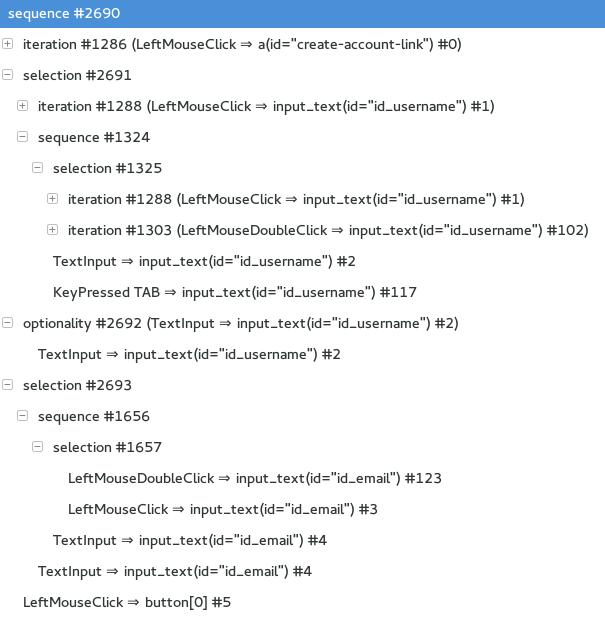
\includegraphics[scale=0.7]{chapters/casestudy/noneventcreateaccount.png}
	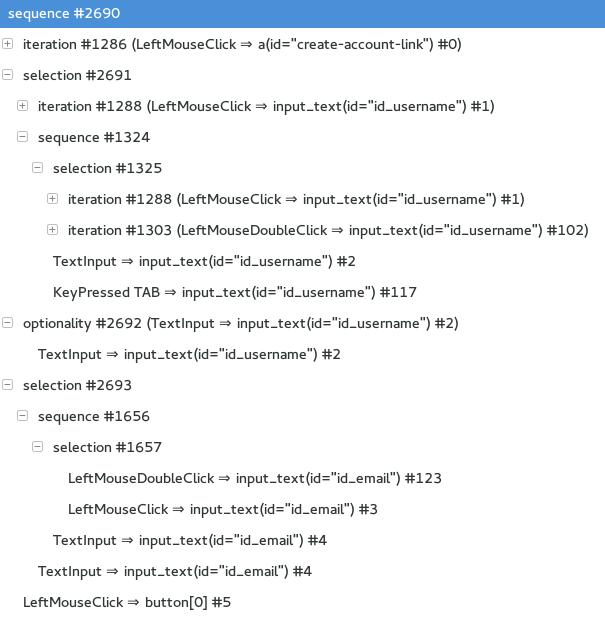
\includegraphics[width=\textwidth]{chapters/casestudy/noneventcreateaccount.png}
	\caption{An example for a task found by alignment task tree generation with distance calculation between non-event-tasks.}
	\label{fig:noneventaccountcreation}
\end{figure}

\begin{table}[h]
	\centering
	\begin{tabular}{l r r}
		\toprule
		&  \multicolumn{2}{c}{\textbf{Testcase}} \\
		\cmidrule{2-3}
		\textbf{Type of non-event-task}& \textbf{with distances}& \textbf{without distances} \\
		\midrule
		Sequences & 352 & 50 \\
		Iterations& 38  & 38 \\
		Selections& 328 & 21 \\
		Optionals & 6   & 8  \\
		\midrule
		\textbf{Performance indicator} & & \\
		\midrule
		Time (s)     & 72.2 & 1.9 \\
		Number of repetitions & 35 & 7\\
		\bottomrule
	\end{tabular}
	\caption{Results of the version with and without calculation of the distances between non-event-tasks}
	\label{tab:resultsnoneventtasks}
\end{table}

\section{Evaluation of termination conditions}
In this section we will investigate if the algorithm for the task tree generation can be terminated with other conditions than the condition mentioned in chapter \ref{chap:approach}.
The described behaviour is that the algorithm stops if no further replacements could be performed.
It has been observed that the most matches are found in the first few repetitions of the sequence detection phase.
Table \ref{tab:timesandmatchesperiteration} and the corresponding figure \ref{fig:hasehase} supports this claim. We can see that the number of matches found in each repetition decreases rapidly.
After the 6th repetition we detect 0.01\% of the matches found in the first sequence detection. We could stop the algorithm here. But since the algorithm finishes shortly after (after the 10th repetiton),
we keep the termination condition for this case study as it is defined in the approach.
If on other case studies the algorithm repeats more often, it can be considered to change the termination condition to a fixed number of iteration.
Another propable condition is to stop when the number of found matches falls below a fraction from the matches found in the first repetition.

We saw in section \ref{sec:noneventtasks} that the number of iterations drastically increases if the distances between non-event-tasks are calculated.
If a good solution for the large computation time of the distances is found, this would be a possible use case of a different termination condition.

\begin{table}[h!]
		\centering
	\begin{tabular}{ l r r r }
		  \toprule
			& & \multicolumn{2}{c}{\textbf{Time (m)}} \\
			\cmidrule{3-4}
		  \textbf{Repetition No.} & \textbf{Matches} & \textbf{Absolute}& \textbf{Relative} \\
		  \midrule
     		 0  & 1,112,794 & 26.17 & 26.17\\
	       1  & 381,190   & 39.16 & 12.99\\
		    2  & 167,677   & 45.52 & 6.36\\
		    3  & 63,964    & 51.00 & 5.48\\
		    4  & 26,171    & 55.83 & 4.83\\
		    5  & 12,627    & 60.72 & 4.89\\
		    6  & 8,660     & 65.48 & 4.76\\
		    7  & 7,517     & 70.34 & 4.86\\
		    8  & 7,232     & 75.02 & 4.68\\
		    9  & 7,214     & 79.74 & 4.72\\
		    10 & 7,214     & 84.49 & 4.75\\
		  \bottomrule
		   \end{tabular}
		   \caption{Matches found per repetition and the time for each repetition. All times in minutes.}
		   \label{tab:timesandmatchesperiteration} %TODO labelanpassen -> repetition
	\end{table}
%
% backing up old table

% \begin{table}[h!]
% 		\centering
% 	\begin{tabular}{|c|r|c|c|}
% 		\hline
% 		\textbf{Iteration No.} & \textbf{Matches} & \textbf{Absolute time}& \textbf{Relative time} \\
% 		\hline
% 					0  & 1,112,794 & 26.17 & 26.17\\
% 					1  & 381,190   & 39.16 & 12.99\\
% 			2  & 167,677   & 45.52 & 6.36\\
% 			3  & 63,964    & 51.00 & 5.48\\
% 			4  & 26,171    & 55.83 & 4.83\\
% 			5  & 12,627    & 60.72 & 4.89\\
% 			6  & 8,660     & 65.48 & 4.76\\
% 			7  & 7,517     & 70.34 & 4.86\\
% 			8  & 7,232     & 75.02 & 4.68\\
% 			9  & 7,214     & 79.74 & 4.72\\
% 			10 & 7,214     & 84.49 & 4.75\\
% 		\hline
% 			\end{tabular}
% 			\caption{Matches found per iteration and the time for each iteration. All times in minutes.}
% 			\label{tab:timesandmatchesperiteration}
% 	\end{table}

	\begin{figure}[h!]
		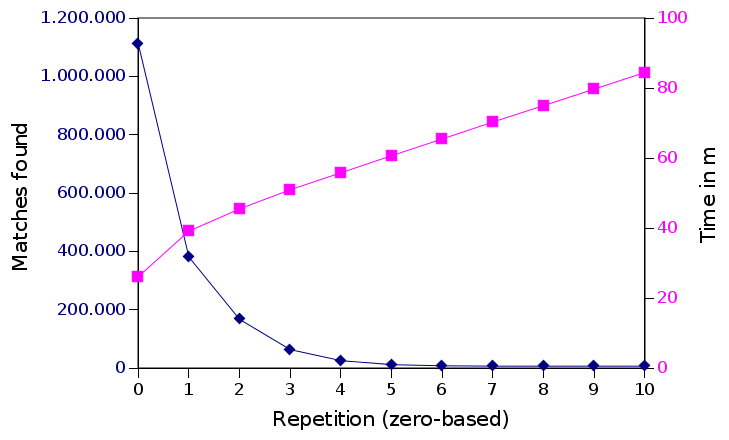
\includegraphics[width=\textwidth]{chapters/casestudy/hasehase.png}
		\caption{}
		\label{fig:hasehase}
	\end{figure}


\section{Performance Evaluation}
To evaluate the performance of the alignment approach we run
\begin{table}[h]
	\centering
\begin{tabular}{|r|r|r|}
	\hline
	\textbf{Count of user sessions} & \textbf{n-gram Approach} & \textbf{alignment approach} \\
	\hline
	  10 & 3.141 & 2.655 \\
	  100 & 12.019 & 5.681 \\
	  1000 & 419.063 & 60.775 \\
	  3602 & 5780.05 & 1,417.37 \\
	\hline
	 \end{tabular}
	 \caption{Comparison between execution times (seconds) of n-gram approach and alignment supported task tree generation}
	 \label{tab:comparisontasktreegenerations}
 \end{table}

 \begin{figure}[h]
	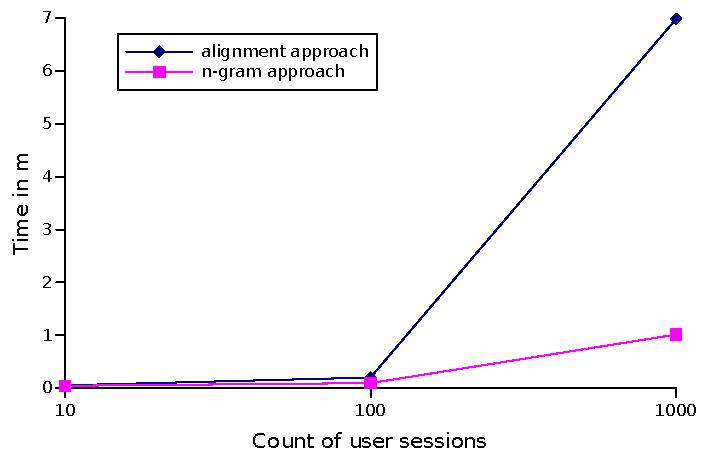
\includegraphics{chapters/casestudy/performance.pdf}
\end{figure}
\section{Generated Task Trees}
\begin{table}
	\centering
 \begin{tabular}{|r|c|c|}
	   \hline
	      & \textbf{n-gram approach} & \textbf{alignment approach} \\
	     \hline
	       \textbf{Generated Tasks} & 10,634 & 6,532 \\
	       Sequences & 9,530 & 2,759 \\
	       Iterations & 1,104 & 619 \\
	       Selections & -& 1,156 \\
	       Optionals & -& 101 \\
	       \hline
\end{tabular}

\end{table}


\begin{itemize}
	\item Show some meaningful generated task trees
	\item Show also tasktrees that are not useful
\begin{figure}
	\centering
	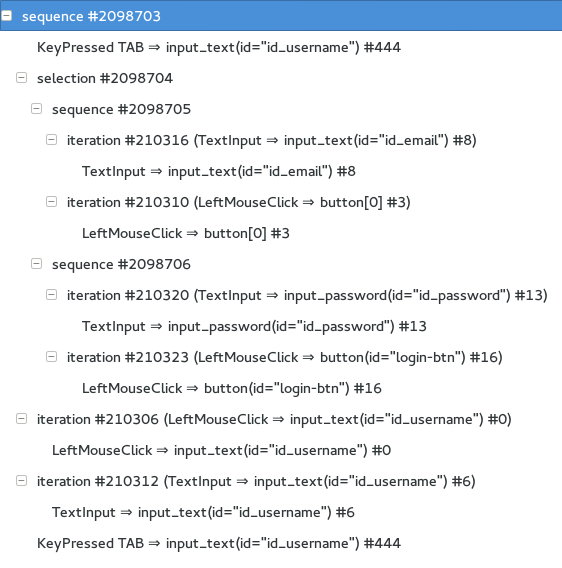
\includegraphics[]{chapters/casestudy/mixedtasktree.png}
	\caption{}
	\label{}
\end{figure}
\begin{figure}
	\centering
	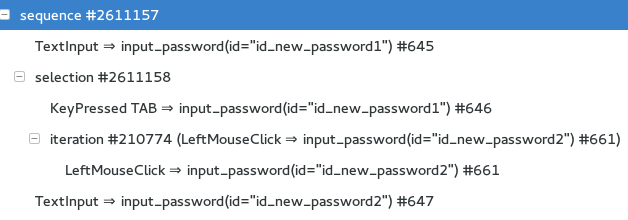
\includegraphics[]{chapters/casestudy/newpassword.png}
	\caption{}
	\label{}
\end{figure}
\begin{figure}
	\centering
	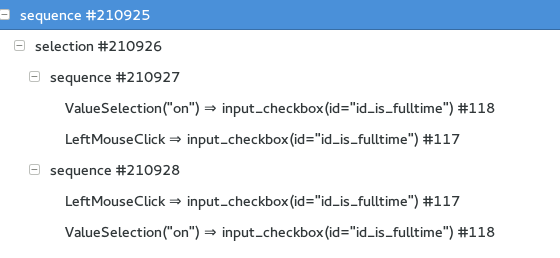
\includegraphics[]{chapters/casestudy/preprocessing_needed.png}
	\caption{}
	\label{}
\end{figure}
\begin{figure}
	\centering
	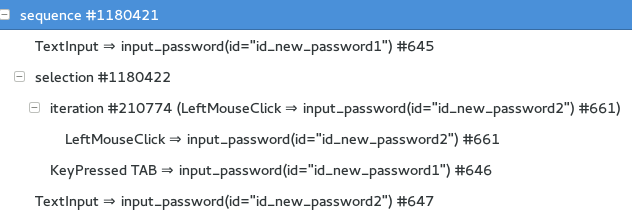
\includegraphics[]{chapters/casestudy/newpassword-1.png}
	\caption{}
	\label{}
\end{figure}
\begin{figure}
	\centering
	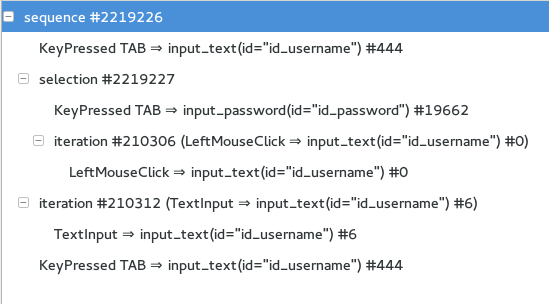
\includegraphics[]{chapters/casestudy/login_process_repeated.png}
	\caption{}
	\label{}
\end{figure}
%\begin{figure}
%	\centering
%	\includegraphics[]{}
%	\caption{}
%	\label{}
%\end{figure}
\end{itemize}


\section{Discussion}
\begin{itemize}
	\item Task Graph
\end{itemize}
